\documentclass[11pt, a4paper]{article}
\usepackage[utf8]{inputenc}
\usepackage[T1]{fontenc}
\usepackage{helvet}
\renewcommand{\familydefault}{\sfdefault}
\usepackage[table]{xcolor}
\definecolor{schoolgreen}{HTML}{92D050}
\usepackage{geometry}
\geometry{margin=2cm, top=4cm, headheight=2.5cm, headsep=0.5cm}
\usepackage{array}
\usepackage{graphicx}
\usepackage{fancyhdr}
\usepackage{amssymb}
\pagestyle{fancy}
\fancyhf{}
\fancyhead[L]{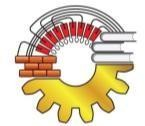
\includegraphics[height=2cm]{../../distritos/4117/templates/logo1.jpg}}
\fancyhead[R]{
\includegraphics[height=2cm]{../../distritos/4117/templates/logo2.jpg}}
\fancyhead[C]{\fontsize{10}{12}\selectfont \textbf{\textit{ESCUELA N.° 4-117 EJÉRCITO DE LOS ANDES \\ DIRECCIÓN DE EDUCACIÓN TÉCNICA Y TRABAJO \\ SECCIÓN V}}}
\renewcommand{\headrulewidth}{0pt}

\begin{document}
\noindent\colorbox{schoolgreen}{\begin{minipage}{\dimexpr\textwidth-2\fboxsep}\centering \textbf{\fontsize{14}{16}\selectfont DIAGNÓSTICO 2026}\end{minipage}}

\vspace{1.5em}
\begin{flushleft}
\textbf{Espacio Curricular:} Prácticas Profesionalizantes \\
\textbf{Año:} 5to \\
\textbf{División:} 3ra \\
\textbf{Profesor/a:} Ferreyra Gustavo David \\
\textbf{Modalidad:} Electromecánica
\end{flushleft}

\vspace{1em}
\noindent \textbf{Marcar las capacidades a evaluar:}

\begin{itemize}
\item $\square$ Observación $\quad$ $\square$ Identificación $\quad$ $\square$ Comparación $\quad$ $\square$ Análisis
\item $\square$ Resumen $\quad$ $\square$ Síntesis $\quad$ $\square$ Clasificación $\quad$ $\square$ Interpretación
\item $\square$ Formulación de críticas $\quad$ $\square$ Búsqueda de suposiciones $\quad$ $\square$ Imaginación y creatividad
\item $\square$ Organización de datos $\quad$ $\square$ Formulación de hipótesis
\end{itemize}

\vspace{1em}
\noindent \textbf{1. Explicitar los aprendizajes específicos evaluados:}
\begin{itemize}
\item Conocimiento y aplicación de normas de seguridad e higiene en el taller.
\item Manejo correcto de herramientas manuales y eléctricas básicas.
\item Capacidad de lectura e interpretación de planos técnicos sencillos.
\item Organización del espacio de trabajo y gestión de residuos.
\end{itemize}

\noindent \textbf{2. Instrumento/s utilizado/s:}
\begin{itemize}
\item Observación directa durante la ejecución de tareas simples en el taller.
\item Lista de cotejo de competencias procedimentales.
\item Entrevista grupal sobre experiencias previas en entornos laborales.
\end{itemize}

\noindent \textbf{3. Descripción de los destinatarios:}
El grupo demuestra una actitud positiva hacia el trabajo práctico y un buen manejo de las herramientas. Se observa una fortaleza en la ejecución manual, pero debilidades en el registro documental de los procesos y en la rigurosidad del orden y limpieza al finalizar la jornada.

\noindent \textbf{4. Alumnos que presentan alguna dificultad:}


\begin{tabular}{|p{0.4\textwidth}|p{0.5\textwidth}|}
\hline
\rowcolor{gray!20} \textbf{Alumnos} & \textbf{Dificultad} \\
\hline
No se registran alumnos con dificultades significativas en esta etapa & N/A \\
\hline
\end{tabular}

\vspace{2em}
\noindent \textbf{Conclusión:}
De acuerdo a lo diagnosticado se podría decir que el grupo está apto para iniciar las prácticas profesionalizantes, enfocando los primeros módulos en la sistematización del registro de tareas y el refuerzo de la cultura de seguridad industrial.
\end{document}